\documentclass{ercisbeamer}

\title{Learning}
\subtitle{Effective Studying}
\author{Sven Ligensa}
\institute{European Research Center for Information Systems (ERCIS)}
\date{\today}


\begin{document}

\setbgimage{00_resources/jungle_brain}
\begin{frame}
    \begin{tbox}
        \titlepage
    \end{tbox}
\end{frame}
\setbgimage{}

\begin{frame}{Contents}
    \tableofcontents
\end{frame}

\setbgimage{04_resources/knowledge_spiral}
\section{Overview}
\begin{frame}{Overview}
    \begin{tbox}
        \begin{itemize}
            \item \red{Learning}: \emph{``\red{Acquiring knowledge} and skills and having them readily available from \red{memory} so you can make sense of \red{future} problems and opportunities.'' \grey{\textasciitilde{} Make It Stick, p. 2}}
            \item \emph{``If you're good at learning, you have an advantage in life.'' \grey{\textasciitilde{} Make It Stick, p. 2}}
            \begin{itemize}
                \item Need to keep learning and remembering \red{for life}
            \end{itemize}
            \item Getting information \red{out} of your brain, \negative{not in} \cite{agarwal19}
            \item \red{Iterative Process}: Revisiting knowledge like a spiral and understanding more every time
            \begin{itemize}
                \item \emph{Can you think of examples?} \pause
                \begin{itemize}
                    \item \emph{Reading a dense paper multiple times: \grey{Some aspects are immediately clear, others not. During the second reading, you build on top of the information have from the first reading.}}
                    \item \emph{Building up on knowledge about \emph{data} or \emph{processes} in subsequent modules: \grey{It would neither make sense to learn all the details in one module, nor to listen to subsequent modules first.}}
                    \item \emph{Refining your notes step-by-step to create a presentation}
                \end{itemize}
            \end{itemize}
            \item On neurological level: Strengthening neural pathways
            \item With right learning techniques: \red{No known limit to how much we can learn and remember if we relate it to what we already know}
        \end{itemize}
    \end{tbox}
\end{frame}

\setbgimage{04_resources/jungle_brain_50}
\section{An Analogy}
\begin{frame}{An Analogy}
    \pause
    \begin{tbox}
        \begin{itemize}
            \item Knowledge $\widehat =$ \red{Tree} \grey{(hierarchical structure)} / \red{Network} \grey{(connections between nodes)}
            \begin{itemize}
                \item Connections: More = Better, Intense = Better
                \item \emph{Can you think of examples?} \pause \emph{$\rightarrow$ Memory of your childhood neighborhood, accident, times of extreme stress}
            \end{itemize}
            \item New learning requires a foundation of \red{prior knowledge}
            \begin{itemize}
                \item Adding to tree of knowledge, requires existing knowledge to connect it to \\ $\rightarrow$ Make information digestible for you
            \end{itemize}
        \end{itemize}
    \end{tbox}
\end{frame}

\setbgimage{04_resources/kurzgesagt}
\begin{frame}{An Analogy}
    \begin{tbox}
        \begin{itemize}
            \item ``Change Your Life - One Tiny Step at a Time'' (\url{https://youtu.be/75d_29QWELk?t=77})
            \begin{itemize}
                \item Video by Kurzgesagt, min 1:17 - 2:10
                \item Brain $\widehat =$ \red{Jungle}: Moving through terrain more often $\Rightarrow$ Easier to do so in the future
                \item Here in the context of building habits, but similar for thinking:
                \begin{itemize}
                    \item Learning $\widehat =$ Gradually enlarging neural pathways
                \end{itemize}
            \end{itemize}
        \end{itemize}
    \end{tbox}
\end{frame}
\setbgimage{}

\section{Forgetting}
\begin{frame}{Forgetting}
    \begin{itemize}
        \item \red{Forgetting}: Inability to recall something (easily)
        \item Learning requires \red{memory}
        \item Central goal: Interrupt the \red{Forgetting Curve}
        \begin{itemize}
            \item We (exponentially) forget most information we consume after a short amount of time
        \end{itemize}
    \end{itemize}

    \begin{figure}
        \centering
        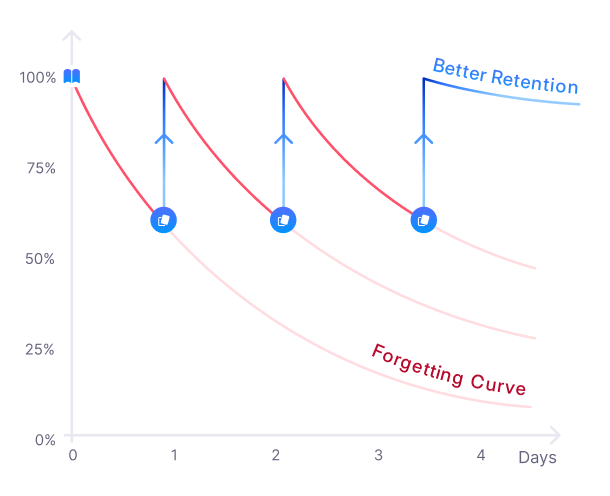
\includegraphics[width=0.35\paperwidth]{04_resources/forgetting_curve_remnote.png}
        \vspace{-0.5em}
        \caption{\tiny \url{https://www.remnote.com/assets/homepage/images/spaced_repetition_retention.webp}}
    \end{figure}
\end{frame}

\section{The Role of Failure}
\begin{frame}{The Role of Failure}
    \begin{itemize}
        \item Source of useful information
        \item Not desirable itself, but unavoidable $\rightarrow$ Effort despite risks
        \item Fear of failure $\Rightarrow$ Worse learning
        \item Important: \positive{Positive attitude} towards mistakes
        \item Few settings where failure not optimal learning strategy
        \begin{itemize}
            \item \emph{Can you think of an example?} \pause \emph{$\rightarrow$ Parachuting}
        \end{itemize}
    \end{itemize}
\end{frame}

\setbgimage{04_resources/own_your_learning}
\section{Own Your Learning}
\begin{frame}{Own Your Learning}
    \begin{tbox}
        \begin{itemize}
            \item \red{Elements shaping your intellectual abilities lie to a large extent within your own control}
            \item \red{Your learning = Your responsibility}
            \item Teachers are there to support you, but at the end, it is up to you how much you learn
        \end{itemize}
    \end{tbox}
\end{frame}

\setbgimage{04_resources/skilltree}
\section{Practice Like an Expert}
\begin{frame}{Practice Like an Expert}
    \begin{tbox}
        \begin{itemize}
            \item \red{Thousands of hours} of \red{deliberate practice} 
            \begin{itemize}
                \item \grey{Debatable: \emph{10,000-Hour Rule} popularized by Malcolm Gladwell}
                \item Goal-directed, often solitary, at edge of current ability (beyond comfort zone $\rightarrow$ often a bit uncomfortable)
            \end{itemize}
            \item Repeated attempts on similar problems
            \item Timely feedback
            \item Valid environments: Regularities which can be learned
            \item Intensity: Quantity $\times$ Quality
            \item \red{Chunking}: Acquisition of increasingly complex patterns
            \begin{itemize}
                \item Analogy: Skill tree in computer games
            \end{itemize}
        \end{itemize}
    \end{tbox}
    \begin{textblock*}{200pt}(130pt, 30pt)
        \tiny \url{https://youtu.be/5eW6Eagr9XA?feature=shared}
    \end{textblock*}
\end{frame}
\setbgimage{}

\section*{Outlook}
\begin{frame}{Outlook}
    \begin{enumerate}
        \item \positive{Introduction}
        \vspace{.5em}
        \item \positive{Illusions of Knowing}
        \item \positive{Understanding the Brain}
        \item \positive{Learning}
        \item Next: \red{Desirable Difficulties}
        \item \grey{Effective vs. Ineffective Learning Strategies}
        \vspace{.5em}
        \item \grey{Retrieval}
        \item \grey{Spacing}
        \item \grey{Variation and Interleaving}
        \item \grey{Mental Models}
        \item \grey{Memory Cues}
    \end{enumerate}
\end{frame}

\thankyou{Happy Learning!}{sven.ligensa@uni-muenster.de}

\sources

\end{document}
